\documentclass[10pt]{article}%\usepackage{esial}

\usepackage[french]{babel}
\usepackage[utf8]{inputenc}
\usepackage{url}
\usepackage{amstext,amsmath,amsfonts,figlatex,fullpage}
\usepackage{fancyvrb}

\title{Le problème de la pyramide}
\author{Julien Le Guen}
\date{Janvier 2006}
\begin{document}

\maketitle

\begin{abstract}
Ce document présente le problème dit de la pyramide et un algorithme pour le résoudre.
Une implémentation (en langage C) de cet algorithme est également présentée en fin du document,
ainsi que les résultats obtenus avec celle-ci.
\end{abstract}

\section{Présentation du problème}
On considère une pyramide la tête en bas de hauteur $n$ comme celle
représentée plus bas. On cherche à remplir toutes les cases avec chacun des
entiers compris entre $1$ et $\frac{n(n+1)}{2}$ en respectant les contraintes
suivantes:
\begin{enumerate}
\item Chaque nombre de $\left[1,\frac{n(n+1)}{2}\right]$ ne figure qu'une fois sur la pyramide
\item La valeur de chaque case est égale à la différence des deux cases placées
  au dessus d'elle.\\
  Ainsi sur la figure~\ref{fig:exemple}, $n_3=|n_1 - n_2|$
\end{enumerate}

\begin{figure}[h]
  \centering
  \includegraphics{fig/pyramide.fig} \vspace{-.5\baselineskip}
  \caption{Exemple de pyramide de hauteur 2.}
  \label{fig:exemple}
\end{figure}

\paragraph*{}
  Certaines instances de ce problème ne connaissent pas de solution. En fait, les seules
  solution connues sont pour les pyramides de taille inférieure à 5 (inclus).
  La littérature sur internet présentant ce problème est très pauvre, et l'auteur ignore
  s'il existe une solution mathématique au problème «Existe-t-il une telle pyramide de taille $n$, 
  avec $n > 5$ ?».

  Nous exposons ici un algorithme assez simple permettant de calculer, si elles existent,
  les pyramides de taille $n$, ainsi que quelques pistes à explorer pour tenter d'accélérer les calculs.


\section*{Représentation mémoire}
  \noindent La première idée pour représenter la pyramide est d'utiliser la
  moitié d'un tableau à deux dimensions et de justifier la pyramide à droite ou
  à gauche.

  Une autre représentation possible prend la forme d'un tableau à une dimension
  en rangeant les différentes «tranches de pyramides» les unes à coté des
  autres. Selon la façon de couper ces tranches, il existe de nombreuses
  manières de numéroter les cases. Les figures \ref{fig:numligne} et
  \ref{fig:numcol} présentent deux numérotations différentes.


\begin{figure}[h]
  \centering
  \includegraphics{fig/ligne.fig}\vspace{-.5\baselineskip}
  \caption{Représentation mémoire.}
  \label{fig:mem}
\end{figure}

\paragraph*{}
  La numérotation par ligne est la première qui vient à l'esprit pour modéliser ce problème.
  Un exemple de numérotation par ligne est donné en figure~\ref{fig:numligne}.
  \noindent Le calcul permettant de calculer l'indice de la case placée sur la \texttt{ligne} et sur
  la \texttt{colonne} est :\\ \centerline{$\dfrac{ligne(ligne-1)}{2}+colonne-1$}\\

  \noindent Le même calcul en utilisant la numérotation par colonne, donnée en figure~\ref{fig:numcol}
  est :\\ \centerline{$\dfrac{colonne(colonne-1)}{2}+ligne-1$}

\begin{figure}[h]
  \begin{minipage}{.45\linewidth}
    \centering
    \includegraphics{fig/pyramide-case-ligne.fig}\vspace{-.5\baselineskip}
    \caption{Une numérotation par lignes.}
    \label{fig:numligne}
  \end{minipage}\hfill
  \begin{minipage}{.45\linewidth}
    \centering
    \includegraphics{fig/pyramide-case-col.fig}\vspace{-.5\baselineskip}
    \caption{Une numérotation par colonnes.}
    \label{fig:numcol}
  \end{minipage}
\end{figure}



\section{Algorithme}
\subsection*{Idée de base}
\paragraph*{}
  La première idée est de générer toutes les pyramides existantes,
  puis de vérifier à postériori si elles vérifient les contraintes ou non.
  Le problème, c'est que l'on génère alors énormément de pyramides fausses,
  car nombre d'entre elles ne respectent pas la deuxième condition.

\paragraph*{}
  Une meilleure approche est de construire la pyramide au fur et à mesure, en s'assurant
  que la partie déjà construite vérifie les deux contraintes. Si on arrive
  à remplir la pyramide de cette façon on est sûr qu'elle est valide.
  On s'apperçoit que la numérotation "par colonne" se prête bien à cette approche. En effet,
  en remplissant la pyramide de gauche à droite en commençant par la case en $(1,1)$,
  la génération de la colonne $n$ ne dépend que du morceau de pyramide à gauche (de
  la colonne $1$ à $n-1$) et du nombre situé en $(1,n)$. Ainsi il suffit de remplir récursivement
  les colonnes de haut en bas et de gauche à droite en respectant les contraintes pour s'assurer
  de la validité de la pyramide générée. Si on ne peut remplir une case de la colonne en respectant
  les contraintes, il suffit de changer le nombre en haut de la colonne pour en recalculer une nouvelle.
  Si on arrive à la dernière case $(n,n)$, le problème admet une solution pour le rang $n$.


\begin{figure}[h]
    \centering
    \includegraphics{fig/pyramide-encours-col.fig}
    \caption{Remplissage partiel par colonnes.}
    \label{fig:encours:col}
\end{figure}

\subsection*{Algorithme}
  L'algorithme utilisé est un simple backtracking, ou parcours d'arbre dont
  on coupe les branches qui à coup sûr n'aboutiront pas à une solution.
  Il retourne la première solution trouvée, si elle existe.\\
  Il utilise la numérotation par colonne et la représentation mémoire linéaire.

  \paragraph*{}
  Le paramètre de la récursion est la colonne $i$ en cours de traitement; la
  condition d'arrêt est le dépassement de la taille de la pyramide : si le
  paramètre \texttt{col} dépasse la hauteur de la pyramide, le problème est
  résolu et la pyramide est complètement correctement résolue.

  Si on parvient à remplir correctement la colonne \texttt{col}, il convient
  de réaliser un appel récursif avec \texttt{col+1} pour tenter de remplir le
  reste de la pyramide. Sinon, on effectue un retour arrière.

  On constate que l'on peut calculer (par une série de soustraction) la
  diagonale entière à partir de la solution partielle et du nombre placé sur la
  première ligne de de la diagonale. La fonction récursive
  \texttt{remplir(col)} consiste donc à tester chaque entier en première
  position de la diagonale, puis à tenter de le «propager», \textit{i.e.} à
  vérifier que la diagonale induite par ce nombre est valide. On échoue si on
  est amenés à réutiliser un nombre déjà utilisé dans la pyramide.

\paragraph*{}
  L'algorithme peut se décrire ainsi :
  \begin{enumerate}
    \item Choix du nombre à placer en haut de la colonne courante $i$
    \item Propagation du choix le long de la colonne $i$
    \item Si on arrive en bas de la colonne $i$, alors récursion sur la colonne suivante $i+1$.
      Si on est en bas de la dernière colonne $n$, alors la pyramide générée est valide, de taille $n$.
    \item Si on ne peut terminer la colonne $i$ en cours du fait des contraintes, on continue la récursion
      avec un autre nombre en haut de la colonne $i$. Si on a utilisé tous les nombres possibles
      pour celle-ci, on revient un cran en arrière dans la récursion et on recommence en $1$ pour la colonne $i+1$.
    \item Si en utilisant tous les nombres possibles en colonne $1$ aucune pyramide valide n'apparait, alors il
      n'existe pas de solution au problème de rang $n$.
  \end{enumerate}

\section{Implémentation}
  Le choix du langage C pour implémenter cet algorithme est naturel, pour sa rapidité d'exécution.
  En effet son caractère récursif le rend très gourmand (il est de complexité en croissance exponentielle).

  Nous avons besoin de construire quelques fonctions utilitaires avant d'écrire l'algorithme, afin de le rendre plus lisible.
  Ces fonctions et procédures étant très simples, le compilateur se chargera de les optimiser 
  (en \textit{inlinant} le code par exemple).

  On peut cependant optimiser le nombre de calculs à effectuer pour vérifier la première contrainte.
  En maintenant en permanence à jour une table des nombres déjà utilisés, il suffit d'un accès à
  la table pour vérifier que le nombre que l'on tente de placer n'est pas déjà pris.
  Pour cela, une petite astuce est de mise: on crée une table de taille \texttt{nb\_elem}, où
  \texttt{nb\_elem} est le nombre d'éléments de la pyramide. On met dans ce tableau les positions
  des différents nombres dans la pyramide. Quand un nombre n'est pas utilisé, on décide qu'il a la position
  \texttt{nb\_elem}. Ceci nous permet de ne faire qu'une comparaison entre la position $p$ du nombre que l'on tente
  de placer et notre position actuelle $a$ dans la pyramide. Si $p > a$ alors le nombre est libre.
  De plus il est inutile de maintenir cette table lors de la remontée récursive (\textit{ie. retirer les nombres
  de la pyramide, c'est-à-dire les mettre en position \texttt{nb\_elem}}) car leur position $p$ est \textit{de facto} supérieure
  à la position courante $a$.

\subsection*{Allocation mémoire}
  Il est nécessaire d'allouer deux tableaux de taille \texttt{nb\_elem}, un pour stocker la pyramide,
  l'autre pour stocker les positions des nombres dans la pyramide. Il faut également initialiser
  le tableau des positions avec la constante \texttt{OUTOFPYR} égale à \texttt{nb\_elem}.
  \begin{verbatim}
int* elements = (int*)malloc(nb_elem * sizeof(int));
int* place = (int*)malloc(nb_elem * sizeof(int));
  \end{verbatim}

  Il ne faudra évidemment pas oublier de libérer la mémoire avant de quitter le programme.
  \begin{verbatim}
free(elements);
elements = NULL;
free(place);
place = NULL;
  \end{verbatim}


\subsection*{Fonctions utilitaires}
  Il nous faut tout d'abord une fonction de calcul de l'indice de la case située en $(lig, col)$.
  \begin{verbatim}
inline int Indice(int lig, int col)
{
    return ((col*(col-1))/2 + lig - 1);
}
  \end{verbatim}

\paragraph*{}
  Puis la fonction qui nous permet de savoir si le nombre que l'on tente de placer est libre ou non.
  \begin{verbatim}
inline int Contains(int val, int lig, int col)
{
    /* On regarde dans la table si val est place avant
     * 1 <= val <= nb_elem */
    return(place[val-1] <= Indice(lig, col));
}
  \end{verbatim}

\paragraph*{}
  Ensuite nous avons besoin d'une procédure pour mettre un nombre dans une case, et d'une fonction
  pour lire le contenu d'une case.
  \begin{verbatim}
inline int ValueAt(int lig, int diag)
{
    return elements[Indice(lig, diag)];
}
  \end{verbatim}

\paragraph*{}
  Enfin, la procédure pour placer un nombre dans une case, qui maintient également la table
  des positions à jour.
  \begin{verbatim}
inline void SetValueAt(int val, int lig, int col)
{
    /* Variables */
    int t,ind;

    /* S'il y a deja un nombre a cette case, on le retire de la liste des pris */
    t = ValueAt(lig, col);
    ind = Indice(lig, col);
    if((t != 0) && (place[t-1] == ind))
        place[t-1] = OUTOFPYR;

    /* On place l'element dans la pyramide */
    elements[ind] = val;

    /* On le marque comme etant pris */
    place[val-1] = ind;

    /* Maintien de la liste des places */
    if(progres < ind+1) progres = ind+1;
}
  \end{verbatim}

\paragraph*{}
  Ceci étant fait, on peut désormais écrire les fonctions qui interviennent directement dans
  la réalisation de l'algorithme.

\subsection*{Construction de la pyramide}
  Nous allons commencer par écrire la fonction qui tente de propager un choix effectué en tête
  de colonne.
  \begin{verbatim}
inline int Propager(int col, int val)
{
    /* Variables */
    int lig, t;

    /* On place val en haut de la colonne */
    SetValueAt(val, 1, col);

    /* Cas trivial */
    if(col == 1) return TRUE;

    /* On essaie de propager sur la colonne */
    for(lig = 2; lig <= col; lig++)
    {
        val = abs(ValueAt(lig-1, col-1) - ValueAt(lig-1, col));
        if(Contains(val, lig, col))
            return FALSE;
        else
        {
            /* On place l'element */
            SetValueAt(val, lig, col);
        }
    }
    /* On a reussi a propager jusqu'en bas */
    return TRUE;
}
  \end{verbatim}

\paragraph*{}
  Ensuite vient la fonction récursive qui teste les nombres et 
  appelle la fonction de propagation pour remplir la pyramide.
  \begin{verbatim}
int RemplirH(int col)
{
    /* Variable */
    int i;

    /* Condition d'arret, on a gagné */
    if(col > hauteur) return TRUE;

    /* On essaie avec chaque valeur */
    for(i = nb_elem; i >= 1; i--)
    {
        if(!Contains(i, 1, col))
        {
            if(Propager(diag, i))
            {
                /* Appel récursif */
                if(RemplirH(diag+1)) return TRUE;
            }
        }
    }
    return FALSE;
}

  \end{verbatim}

\paragraph*{}
  Il ne nous manque plus que la fonction qui va initialiser la récursion.
  C'est cette fonction que l'on appellera dans le corps du programme principal
  pour calculer les solutions du problème.
  \begin{verbatim}
void Remplir(void)
{
    /* On commence par la premiere diagonale */
    RemplirH(1);
}
  \end{verbatim}

  L'ensemble des fonctions nécessaires au bon déroulement de l'algorithme étant
  données, nous laissons le soin au lecteur de réaliser le programme qui va autour
  pour lancer le calcul.

\section{Résultats}
  Cette section présente les résultats que nous avons obtenus avec cette implémentation.
  Nous verrons ainsi l'effet dévastateur d'une exponentielle sur le temps de calcul.
  Pour obtenir ces résultats, nous avons ajouté un chronomètre et mémorisé la position
  atteinte lors du calcul de la meilleure pyramide, afin de voir jusqu'où il est possible
  de remplir les pyramides qui n'acceptent pas de solution.

  A ce jour, nous n'avons pu explorer que les problèmes de rang $1$ à $12$.
  Les seuls problèmes admettant une solution sont ceux de rang inférieur ou égal à $5$.
  Nous ne savons pas s'il existe une solution pour les rangs supérieurs, mais les relevés
  nous laissent à croire que ça n'est peut-être pas le cas, sans pour autant en avoir la certitude.

  Pour indication, les calculs jusqu'au rang 11 ont été menés sur un centrino 1.5GHz.
\paragraph*{}
\begin{figure}[h]
\centering
\begin{tabular}{|r|r|r|r|r|}
\hline
Rang & Nb cases & Nb remplies & Taux & Temps (en s)\\
\hline
2 & 3 & 3 & 100,00\% & 0,0020\\
3 & 6 & 6 & 100,00\% & 0,0020\\
4 & 10 & 10 & 100,00\% & 0,0030\\
5 & 15 & 15 & 100,00\% & 0,0060\\
6 & 21 & 20 & 95,24\% & 0,1200\\
7 & 28 & 25 & 89,29\% & 0,9000\\
8 & 36 & 31 & 86,11\% & 6,0000\\
9 & 45 & 37 & 82,22\% & 70,0000\\
10 & 55 & 43 & 78,18\% & 948,0000\\
11 & 66 & 49 & 74,24\% & 11551,0000\\
12 & 78 & 57 & 73,08\% & 103671,0000\\
\hline
\end{tabular}
\caption{Relevé pour les rangs 1 à 12.}
\label{tab:releve}
\end{figure}

\paragraph*{}
Ce relevé nous permet de dresser les courbes suivantes (figure~\ref{fig:temps_normal}
et figure~\ref{fig:temps_semilog}).
\begin{figure}[h]
\centering
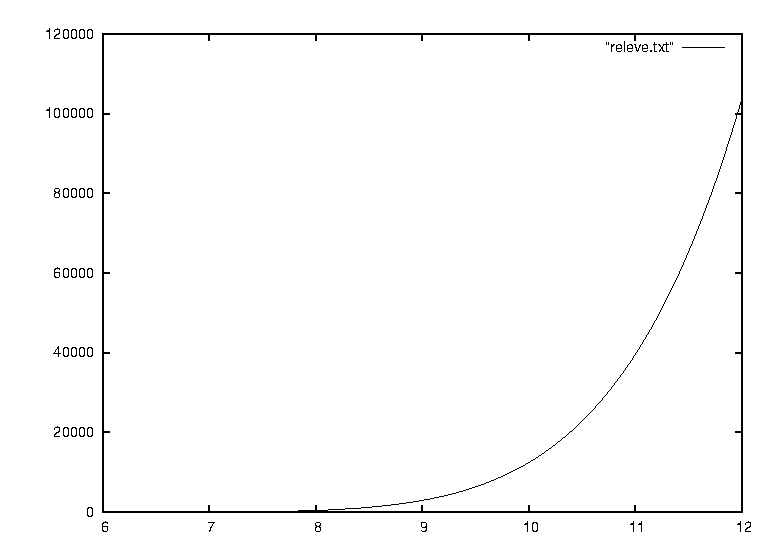
\includegraphics{fig/temps_normal.eps}
\caption{Temps de calcul en fonction du rang}
\label{fig:temps_normal}
\end{figure}
\begin{figure}[h]
\centering
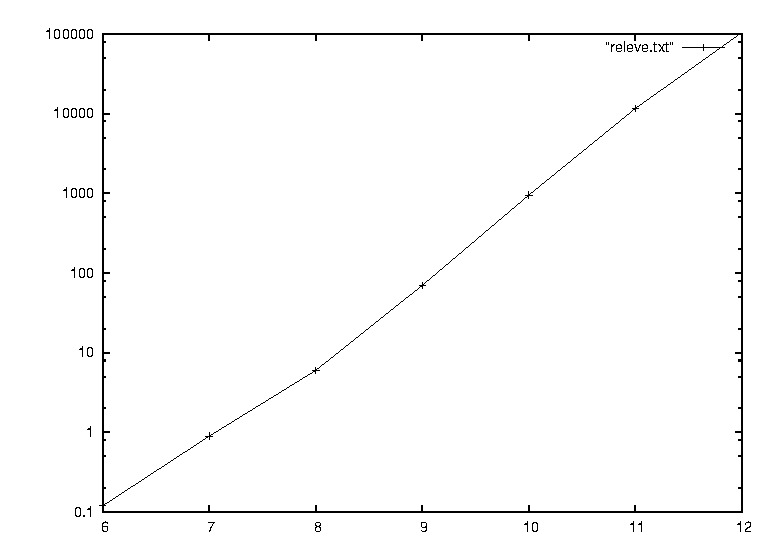
\includegraphics{fig/temps_semilog.eps}
\caption{Temps de calcul en fonction du rang (semilog)}
\label{fig:temps_semilog}
\end{figure}

La figure~\ref{fig:temps_semilog} met en évidence le caractère exponentiel de l'algorithme
utilisé, et nous permet d'extrapoler sur les temps de calcul des problèmes de rang $n > 12$.
Il y a en effet un facteur $10$ entre le temps de calcul du rang $n$ et celui du rang $n+1$,
ce qui nous amène à approximativement 12 jours pour traiter le problème de rang $13$.

Ces constatations nous ont amené à envisager la distribution des calculs en utilisant plusieurs
ordinateurs en même temps pour réduire le temps de calcul.


\section{Distribution du calcul}
L'algorithme est facilement «parallèlisable» de par sa nature combinatoire.
Une version «parallèlisée» du programme a donc été concue, afin de pouvoir le déployer
sur plusieurs machines en même temps.

Il suffit de modifier une seule et unique fonction, celle qui initie la récursion.
Elle prend maintenant pour paramètre la \texttt{valeur} à mettre dans la première colonne,
et initie la récursion sur la deuxième colonne. En déployant le programme modifié sur
plusieurs machines et en leur demandant de calculer les solutions avec une \texttt{valeur}
différente pour chacun, le problème sera traité entièrement mais plus rapidement.
\begin{verbatim}
void Remplir(int valeur)
{
    /* On met la valeur dans la première case */
    SetValueAt(valeur, 1, 1);
    /* On commence par la deuxième diagonale */
    RemplirH(2);
}
\end{verbatim}


\section{Quelques pistes pour aller plus loin}
Malgré cela, l'algorithme reste très gourmand en mémoire, et nous ne pourrons gagner qu'un ou deux
rangs en un temps «raisonnable».
\paragraph*{}
Nous n'avons exploré qu'une seule possibilité de représentation mémoire. On devrait pouvoir s'affranchir
de la multiplication dans la fonction \texttt{Indice}, qui est appelée un très grand nombre de fois,
en simplifiant la structure de donnée représentant la pyramide. Ainsi un tableau à deux dimensions,
contenant la pyramide (justifiée à droite par exemple) et un tableau de pointeurs vers le début
de chaque ligne de la pyramide devraient pouvoir accélérer les calculs en utilisant uniquement
des additions pour accéder aux cases de la pyramide.

\paragraph*{}
Une autre méthode de résolution du problème serait de changer d'algorithme, et d'utiliser la première
idée évoquée plus haut, c'est à dire utiliser la représentation mémoire linéaire et générer les
combinaisons possible, mais en vérifiant la validité de la solution au cours de la génération, et non
à la fin. Cela permettrait de passer de $O(n^2 n!)$ en $O(e^n)$, comme l'algorithme précédent, mais
les optimisations seront peut-être plus aisées.



\section{Bibliographie et autres formes du problème}
Le site \url{http://jeuxmaths.free.fr/c2eno.htm} présente ce problème (parmis
d'autres) sous la formulation suivante :
\begin{quote}
  \textbf{Enigme du billard}

  Si on cherche à disposer en triangle les 15 boules, numérotées de 1 à 15,
  d'une partie de billard américain de façon que chaque boule (sauf celles
  situées sur la 1ère ligne) soit la différence des 2 boules situées
  immédiatement au-dessus, on pourrait trouver la disposition suivante :

  13 3 15 14 6\\
  10 12 1 8\\
  2 11 7\\
  9 4\\
  5

  (la solution est unique à une symétrie près)

  \textit{Généralisons} : Avec une pyramide de n étages, on peut chercher à
  placer les n(n+1)/2 premiers entiers toujours de façon à ce qu'ils obéissent
  à la même règle. Et si cela semble impossible avec $n>5$, alors on peut
  chercher à minimiser le plus grand nombre utilisé ! Et ... c'est ce qui vous
  est demandé pour n = 8.  En résumé : il s'agit de minimiser le plus grand
  nombre utilisé dans une pyramide à 8 étages n'utilisant que des nombres
  entiers strictement positifs distincts tels que chaque boule (sauf celles
  situées sur la 1ère ligne) soit la différence des 2 boules situées
  immédiatement au-dessus.
\end{quote}

Cette extension offre de nouvelles perspectives puisque le problème de base ne
semble pas admettre de solutions pour $n>5$. 

\end{document}
%%% Local Variables:
%%% coding: utf-8
